%%%%%%%%%%%%%%%%%%%%%%%%%%%%%%%%%%%%%%%%%%%%%%%%%%%%%%%%%%%%%%%%%%%%%%%%%%%%%%%%
%2345678901234567890123456789012345678901234567890123456789012345678901234567890
%        1         2         3         4         5         6         7         8
\documentclass[letterpaper, 10 pt, conference]{ieeeconf}  % Comment this line out
                                                          % if you need a4paper
%\documentclass[a4paper, 10pt, conference]{ieeeconf}      % Use this line for a4

\usepackage{float}
                                                          % paper
% uso paquete bookmark para tener bien los outlines.
\usepackage{bookmark}

% Configuro el idioma.
\usepackage[utf8]{inputenc} % Importante para mantener acentos.
\usepackage[spanish, activeacute]{babel} % Requiere: texlive-lang-spanish. Por primera vez hay que ejecutar: texconfig init> log

% Paquete para poder usar acentos en $$.
\usepackage{mathtools}
%\setmathfont{XITS math}

% package to get \url
\usepackage{hyperref}
\hypersetup{
  colorlinks=true,
  linkcolor=magenta,
  filecolor=magenta,
  citecolor=magenta,      
  urlcolor=magenta,
}

% Graficos electrónicos
\usepackage{circuitikz}

\IEEEoverridecommandlockouts                              % This command is only
                                                          % needed if you want to
                                                          % use the \thanks command
\overrideIEEEmargins
% See the \addtolength command later in the file to balance the column lengths
% on the last page of the document

\usepackage{graphicx}
\usepackage{graphics}

% styling for matlab/octave code.
\usepackage{matlab-prettifier}
% Configuracion, con esto puede agregar ñ.
\lstset{
  literate={ñ}{{\~n}}1
}

% The following packages can be found on http:\\www.ctan.org
%\usepackage{graphics} % for pdf, bitmapped graphics files
%\usepackage{epsfig} % for postscript graphics files
%\usepackage{mathptmx} % assumes new font selection scheme installed
%\usepackage{times} % assumes new font selection scheme installed
\usepackage{amsmath} % assumes amsmath package installed
%\usepackage{amssymb}  % assumes amsmath package installed

\title{\LARGE \bf Laboratorio N° 1}

\author{
  Tom\'as Vidal\\
  {\it Circuitos Electrónicos 1}\\
  {\it Facultad de Ingenier\'ia, UNLP, La Plata, Argentina.}\\
  {\it 26 de Marzo, 2024.}
}                                            % <-this % stops a space


% comienzo

% INTRO


% Figura
\newcommand{\image}[2] {
  \begin{figure}[H]
    \centering
    \includegraphics[width=0.43\textwidth]{./#1.png}
    \caption{#2}
    \label{fig:#1}
  \end{figure}
}

% Codigo
% \begin{lstlisting}[style=Matlab-editor]
% % el código va aca
% dispc("HELLO WORLD");
% \end{lstlisting}

\begin{document}
\maketitle
\thispagestyle{empty}
\pagestyle{empty}

\section{INTRODUCCCI\'ON}
A continuación se detallan los procedimientos y resultados del laboratorio de Circuitos Electrónicos 1. Se emplearon dos configuraciones para un amplificador operacional (\textit{inversora} y \textit{no inversora}), se efecturaron análisis de frecuencias y ganancias para diferentes valores de los componentes involucrados, los mismos se especifican en los resultados. Se concluye que el producto de ganancia ancho de banda se conserva para una misma topología. Posteriormente se realizaron pruebas sobre una placa de ensayo en la que aparecían no linealidades, y luego de activar la realimentación desde la salida se solucionó la no linealidad.

\section{Topologías empleadas}
\subsection{Elementos de trabajo}
Para realizar las pruebas se emplearon diversos instrumentos de laboratorio: \textit{osciloscopio}\footnote{Instrumento utilizado para visualizar y analizar formas de onda eléctricas.}, \textit{multímetro}\footnote{Dispositivo que se utiliza para medir magnitudes eléctricas como corriente, voltaje y resistencia.}, \textit{fuente regulable}\footnote{Dispositivo que proporciona una corriente o voltaje de salida regulable y estable.}, \textit{generador de funciones}\footnote{Dispositivo utilizado para generar señales eléctricas de forma controlada (en amplitud y frecuencia), como ondas sinusoidales, cuadradas, etc. }, y las placas de ensayos provistas a las cuales se las referirá como \textit{1} (\ref{placaDePruebas1})\footnote{Breve descripción de la placa de ensayo 1.} y \textit{2} (\ref{placaDePruebas2})\footnote{Breve descripción de la placa de ensayo 2.}. 

\subsection{Placa de ensayos 1}
La placa de ensayos \textbf{1} permite recrear diversas topologías de una etapa de amplificación con un amplificador operacional 741\footnote{Para ver las especificaciones vea la hoja de datos del fabricante \href{https://www.ti.com/lit/ds/symlink/lm741-mil.pdf}{https://www.ti.com/lit/ds/symlink/lm741-mil.pdf}}, esta placa es la síntesis correspondiente al diagrama circuital de la figura \ref{diagramaPlaca1}. En particular se trabajó con las topologías realimentadas negativamente (realimentación por entrada no inversora) de tal manera que una de ellas sea inversora \ref{diagramaConfigInversora} (es decir crea un desfase de 90°) y otra no inversora \ref{diagramaConfigNoInversora} (no hay desfase).
\begin{figure}[H]
  \centering
  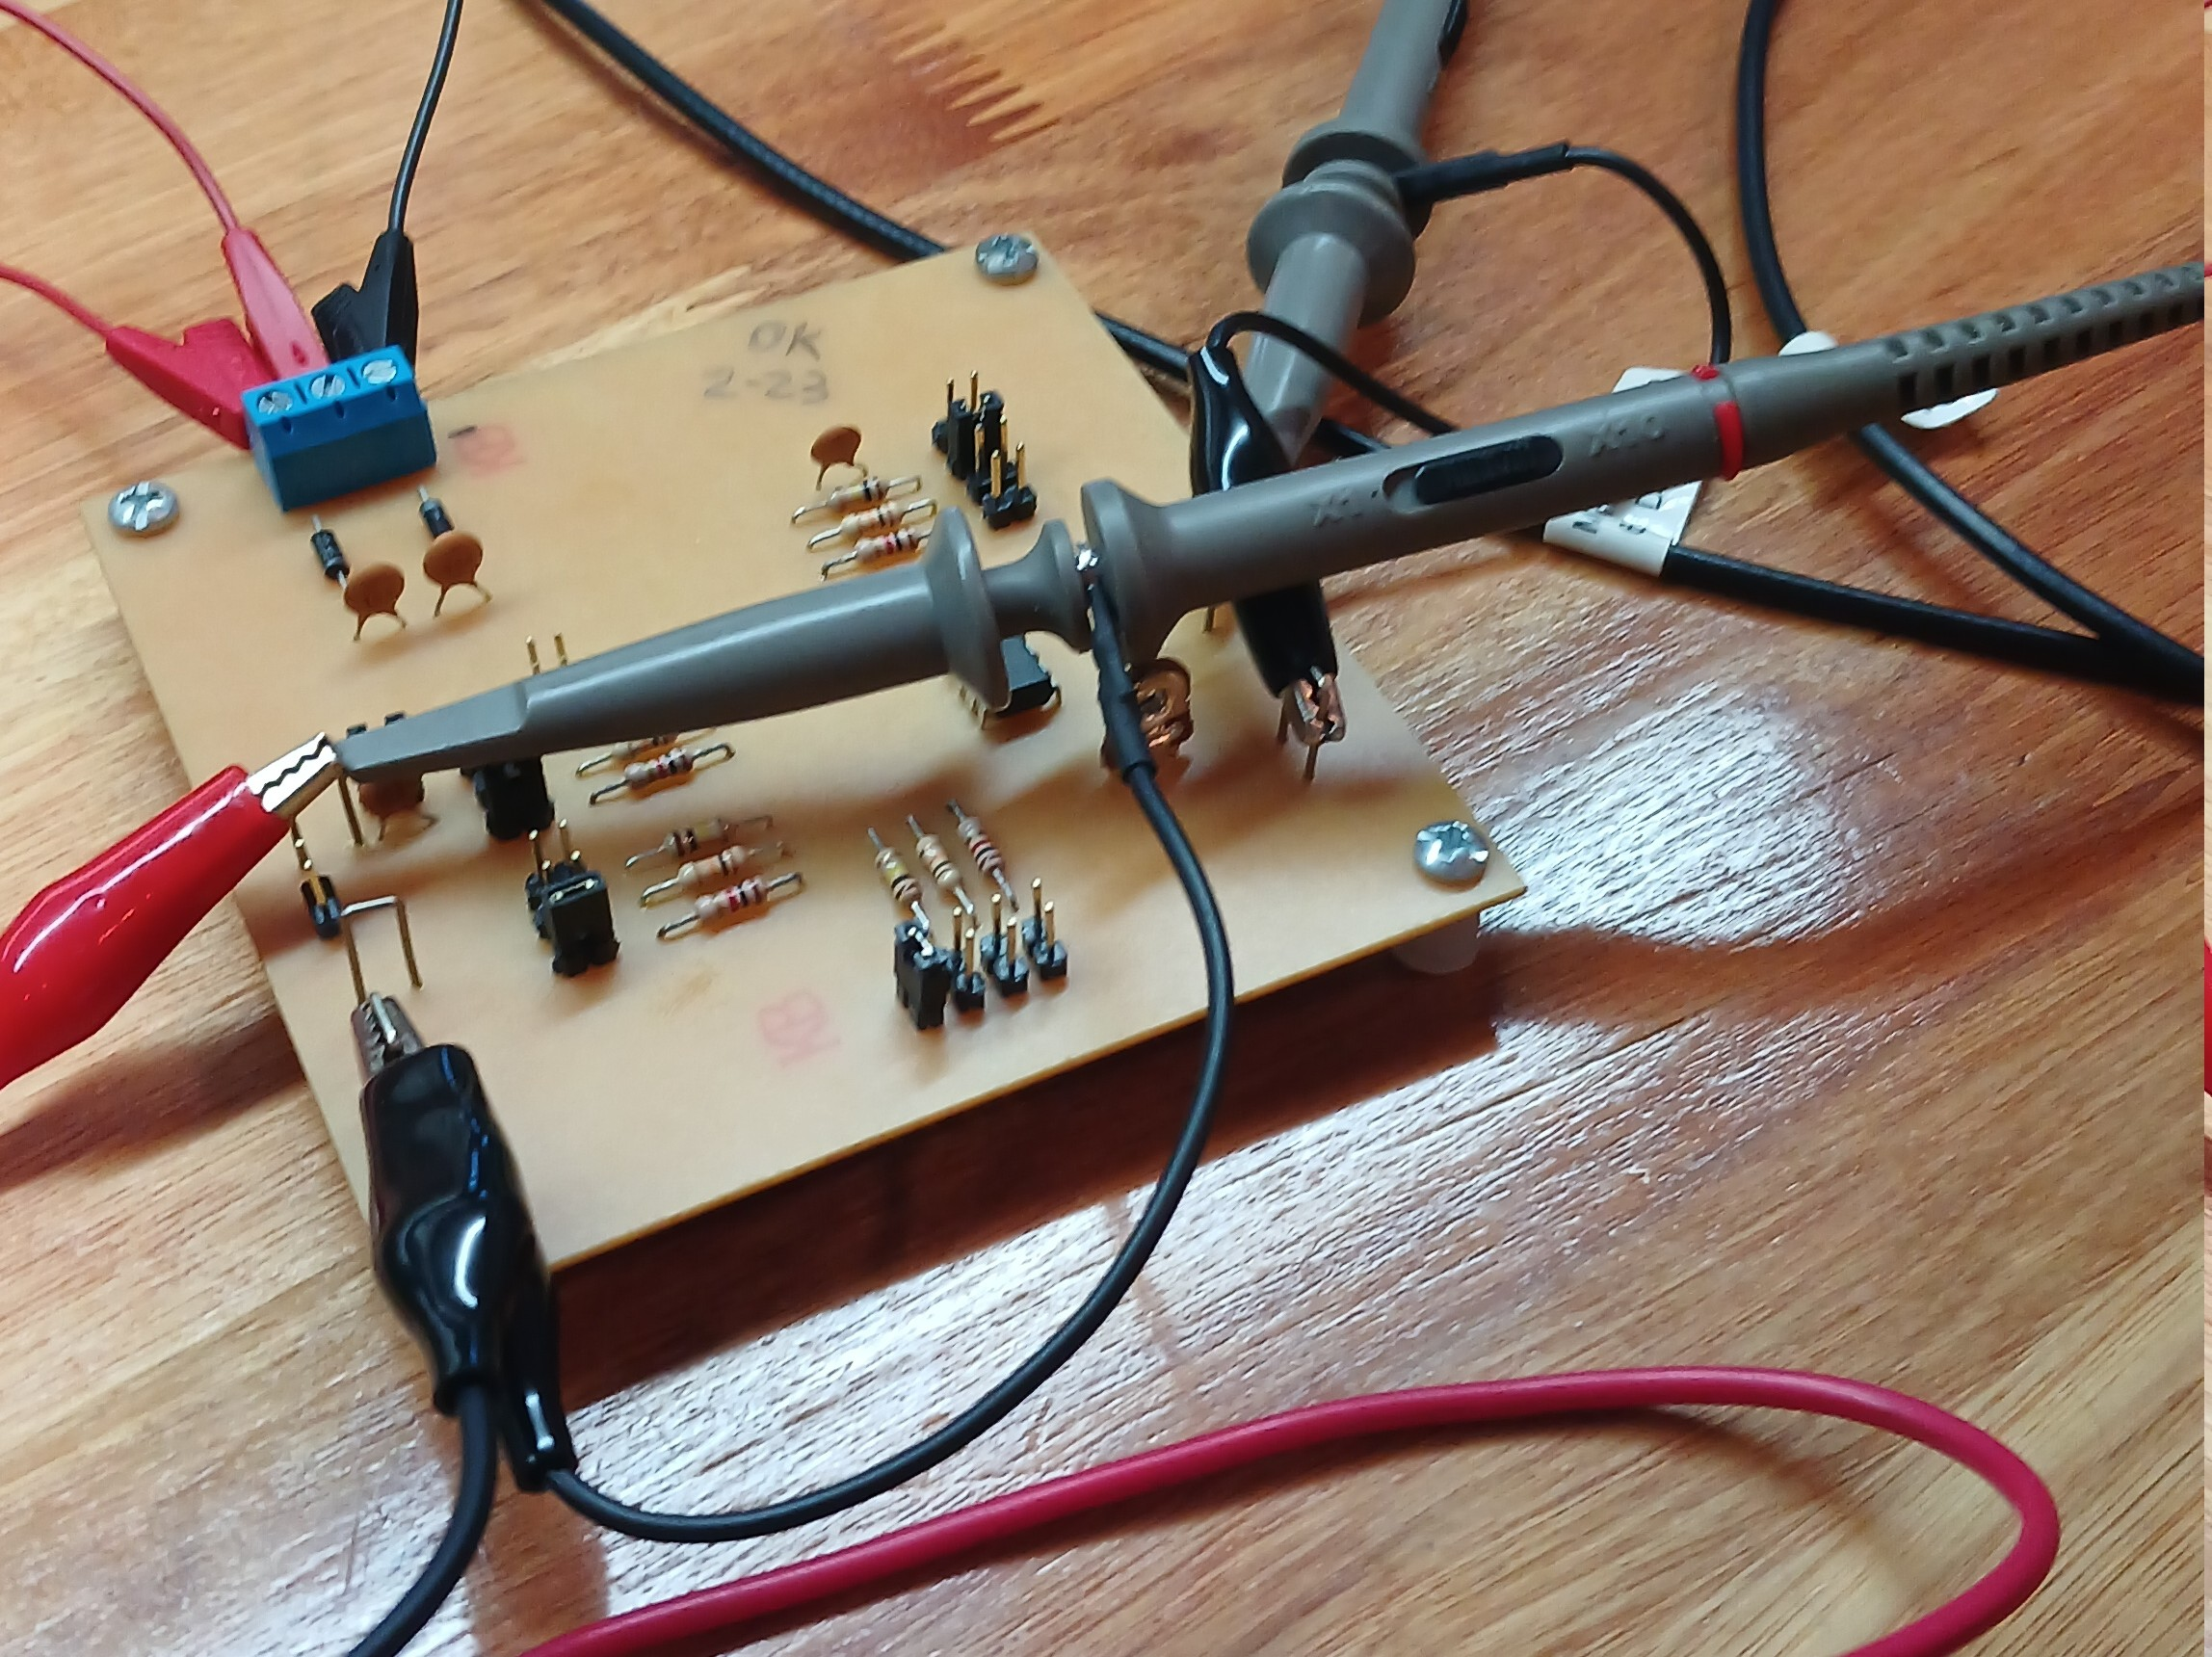
\includegraphics[width=0.43\textwidth]{./placaDePruebas1.jpg}
  \caption{Diagrama correspondiente a la placa de ensayos 1}
  \label{placaDePruebas1}
\end{figure}
\begin{figure}[H]
  \centering
  % TODO
  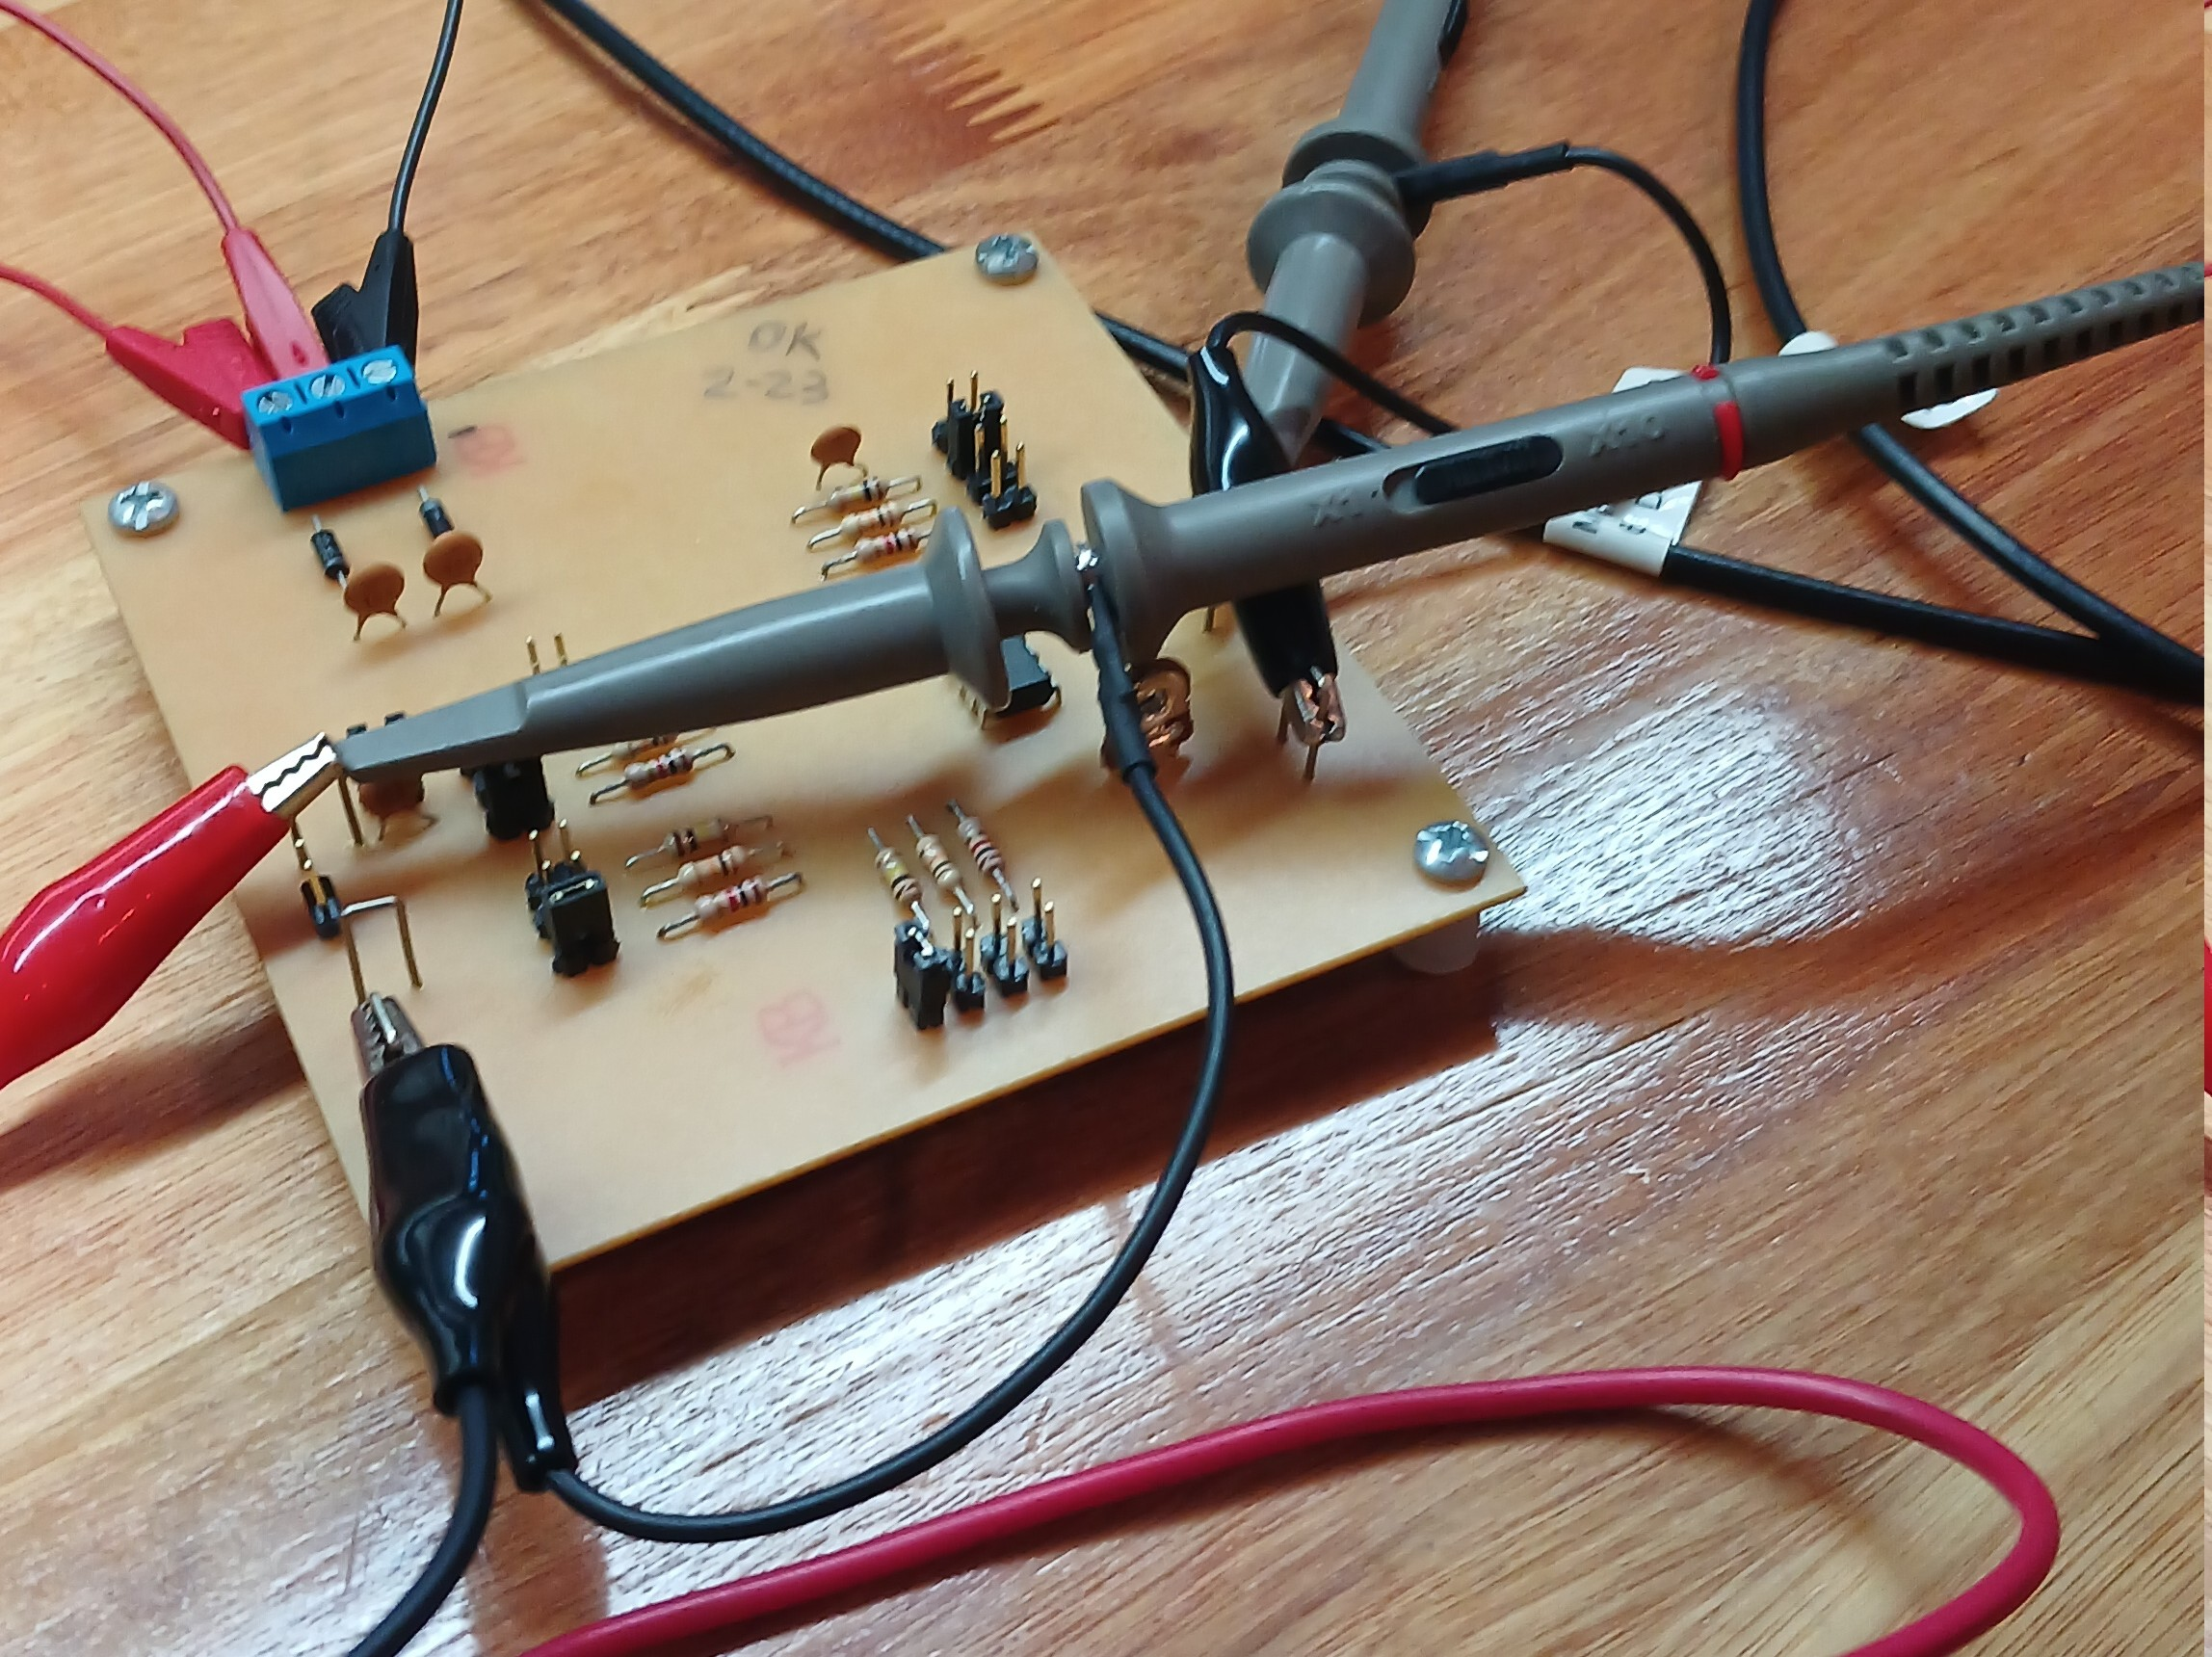
\includegraphics[width=0.43\textwidth]{./placaDePruebas2.jpg}
  \caption{Diagrama correspondiente a la placa de ensayos 1}
  \label{placaDePruebas2}
\end{figure}

Para poder construir estas topologías se configuraron los \textit{jumpers}\footnote{Un \textit{jumper} o \textit{puente} es un elemento de electrónica que permite abrir o cerrar un circuito eléctrico mediante terminales.} de la placa de pruebas 1. Posteriormente se midió la entrada y la salida del circuito con las sondas del osciloscopio, canal 1 en la entrada (\textit{color amarillo en la pantalla}) y el 2 en la salida (\textit{color azul en la pantalla}). Luego se conectó a la entrada el generador de señales y se alimentó la placa (+12V, GND y -12V) con la fuente regulable. De esta manera se pudo analizar la ganancia y la frecuencia de corte de -3dB del amplificador para diferentes valores de los resistores involucrados y en las dos topologías (inversora y no inversora).

\subsection{Resultados de la topología inversora}


\begin{figure}[H]
   \centering
   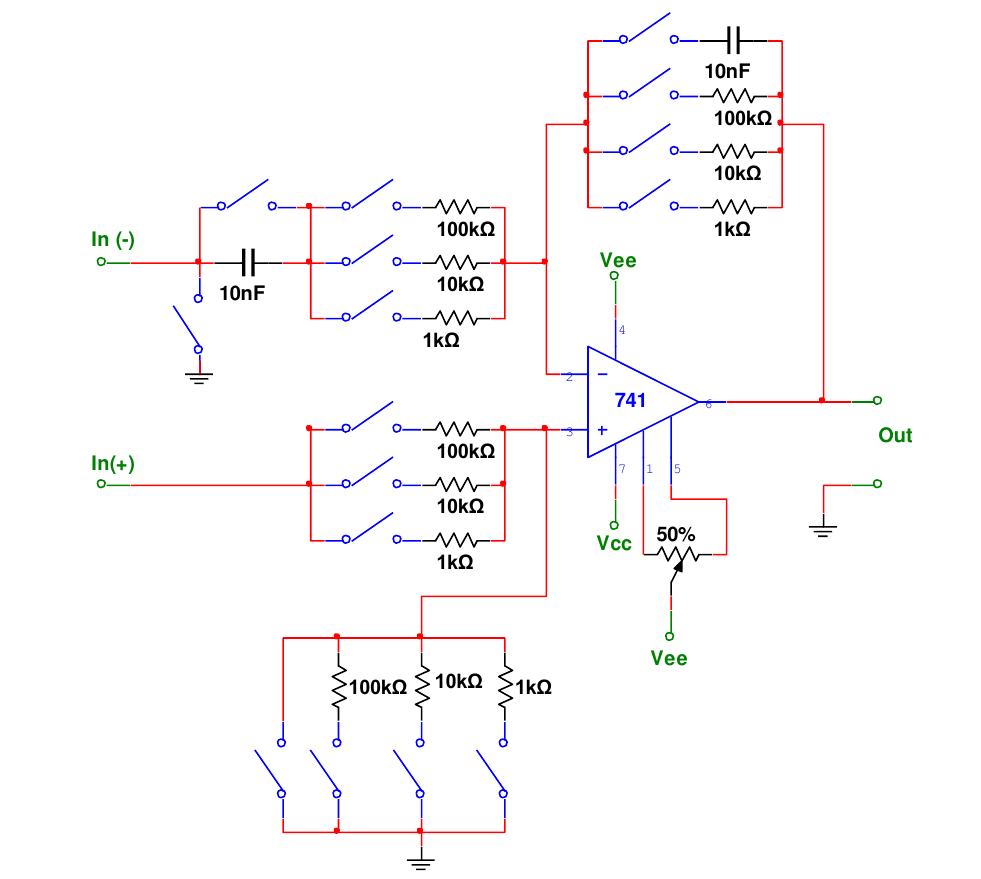
\includegraphics[width=0.43\textwidth]{./diagramaPlaca1.png}
   \caption{Diagrama correspondiente a la placa de ensayos 1}
   \label{diagramaPlaca1}
 \end{figure}

\begin{figure}[H]
  \centering
  \begin{circuitikz}
    \node[op amp] (opamp) at (0,0) {};
    \draw (opamp.+) -- ++(-0.25,0) -- ++(0,-0.5) node[ground]{};
    \draw (opamp.-) -- ++(-1,0) to[R=$R_1$] ++(-1.5,0) -- ++(-0.5,0) node[ocirc]{} coordinate (Vin) node[left] {$V_{in}^{+}$};
    \draw (opamp.out) -- ++(0.25, 0) node[circ]{} -- ++(0,2) -- ++(-0.5,0) to[R=$R_f$] ++(-2,0) -- ++(-0.25,0) -- ++(0,-1.5) node[circ]{};
    \draw (opamp.out) -- ++(1, 0) node[ocirc]{} coordinate (Vout) node[right] {$V_{out}^{+}$};
  \end{circuitikz}
  \caption{Amplificador operacional en configuración inversora}
  \label{diagramaConfigInversora}
\end{figure}
\begin{figure}[H]
  \centering
  \begin{circuitikz}
    \node[op amp] (opamp) at (0,0) {};
    \draw (opamp.+) -- ++(-1,0) node[ocirc]{} coordinate (Vin) node[left] {$V_{in}^{+}$}; 
    \draw (opamp.-) -- ++(-1,0) to[R=$R_1$] ++(-2,0) node[ground]{};
    \draw (opamp.out) -- ++(0.25,0) -- ++(0,2) -- ++(-0.5,0) to[R=$R_f$] ++(-2.5,0) -- ++(0,-1.5) node[circ]{};
    \draw (opamp.out) -- ++(0.25,0) node[circ]{} -- ++(1,0) node[ocirc]{} coordinate (Vout) node[right] {$V_{out}^{+}$};
  \end{circuitikz}
  \caption{Amplificador operacional en configuración no inversora}
  \label{diagramaConfigNoInversora}
\end{figure}
\subsection{Topología inversora}

\begin{thebibliography}{99}

% TODO
\bibitem{tftd_tp5}TODO
% \bibitem{tftd_tp5}ANÁLISIS DE SISTEMAS Y SE\~{n}ALES - A\~{n}O 2022, Práctica 5 Transformada de Fourier de Tiempo Discreto (TFTD), Serie Discreta Fourier (SDF).
% \bibitem{tftd_teoria}ANÁLISIS DE SISTEMAS Y SE\~{n}ALES - A\~{n}O 2022, Filminas de teor\'ia 5: Transformada de Fourier de Tiempo Discreto (TFTD).
%
\end{thebibliography}

\end{document}
